\begingroup
\RaggedRight

\begin{quote}
"Chaos: When the present determines the future, but the approximate present does not approximately determine the future."
\newline
\hfill  — \textit{Edward Lorenz, The Essence of Chaos}
\end{quote}

\section*{Introduction}\label{sec1}
The number of wearable devices have increased exponentially in the recent times and is expected to exceed more than \$67 Billion by 2024 \cite{9214833}. Much like embedded devices, they are loaded with sensors for collecting data from the surrounding ecosystem and transmitting the data to the destination for desired analysis and actions. With the advancement in healthcare wearable devices \cite{wang2022cloud} such as implantable pacemakers, biofluidic-based wearables, and skin-based wearables, there has been growing concern over their manufacturing and their implications for security and privacy \cite{wen2021quantum}. Consider a pacemaker as an example. If an eavesdropper gets access to the data, it creates a privacy issue for the user \cite{al2022medical}, but if the receiver's circuit is duplicated, the attacker can decode the data and pose a life-threatening threat by sending malicious actions to the pacemaker. Therefore, not only is a solution needed for reliable communication resistant to eavesdropping, but also the risk-sensitive issues of device duplication must be addressed.  

Because chaos-based communication \cite{zhong1985experimental, hedayatipour2021comprehensive} is highly sensitive to initial conditions and synchronize over time, it is a suitable choice for reliable communication \cite{duan2022fully} against eavesdroppers. Moreover, use of chaos is suggested as a potential alternative in post-quantum cryptography \cite{onuki2022secret}. Although there are improvements over chaotic communication, for example, the implementation of hyperchaotic circuits \cite{zhang2022hyperchaotic}, not much work has been done to secure the design and manufacturing of chaotic transceivers at an untrusted foundry \cite{rezaei2019hybrid}. Due to the growing trend in outsource manufacturing, the electronic industry must deal with various hardware threats that an untrusted foundry can pose. Since the third-party foundry has access to the circuit design, it can do a lot of unintended activities, which not only have a negative impact on the designers' revenues but, more importantly, can be risk-sensitive to end users, especially in the case of healthcare wearable and implantable devices. One approach to addressing untrusted foundries is to implement logic locking (a.k.a. logic encryption) on the circuits. Logic locking \cite{Koushanfar-LL} is a mechanism to enable the desired behavior of the circuit only when the correct key is applied to the circuit. Recently, Register-Transfer Level (RTL) locking is proposed to protect sensitive Intellectual Property (IP) semantics against untrusted entities \cite{limaye2021fortifying}. However, this approach is not suitable for mixed-signal circuits like transceivers. Moreover, different chaos-based implementations of basic logic gates to obfuscate power profiles and mitigate power analysis–based side channel attacks are proposed \cite{8383903,8383903journal}, and the concept of asymmetry in chaotic Boolean gates is exploited to lock the circuit \cite{9424321}; but the main goal of these initiatives is to use the unique features of chaos to reach hardware security goals in digital circuits rather than proposing secure and reliable mixed-signal chaotic transceivers. In addition, an approach to securing mixed-signal circuits via logic locking is proposed \cite{8715043}, which relies on logic locking of the digital portion of the mixed-signal IC such that unless the correct digital key is provided, the mixed-signal performance will be pushed outside of the acceptable specification range. However, directly locking the analog portion of the mixed-signal ICs via an analog key has not been investigated.

Thus, in this paper, we use a low-overhead yet effective approach to enable logic locking using memristors \cite{chua1971memristor} in the chaotic circuits. We believe that memristor, as the fourth fundamental two-terminal circuit element, can close the gap between reliable communication and secure manufacturing since its resistance can be programmed by the designer and not the foundry.

Fig. \ref{fig:Logic-locked} shows our proposed solution to address the issue of untrusted foundries and eavesdroppers together. On a logic-locked Chua's chaotic circuit, an input signal is encrypted and sent over a public channel. The encrypted signal is decoded at the receiver, which is also logic-locked, and only with the correct key values for the memristor can the message be successfully decoded. Because chaotic maps are highly sensitive and the key space is exponentially large, logic locking based on memristors makes it safe against an attacker attempting to duplicate the receiver without knowing the correct key value. The key contributions of this work are threefold:
\begin{itemize}
   \item Establishing reliable communication against eavesdroppers using memristor-based Chua's chaotic system;
    \item Proposing a novel logic locking mechanism based on the use of memristors as the keys for securing the circuit design against untrusted foundries;
    \item Practical realization of the proposed system on LTSpice and NI Multisim; and validating the system of equations in MATLAB Simulink.
\end{itemize}

\begin{figure}[!t]
    \centering
    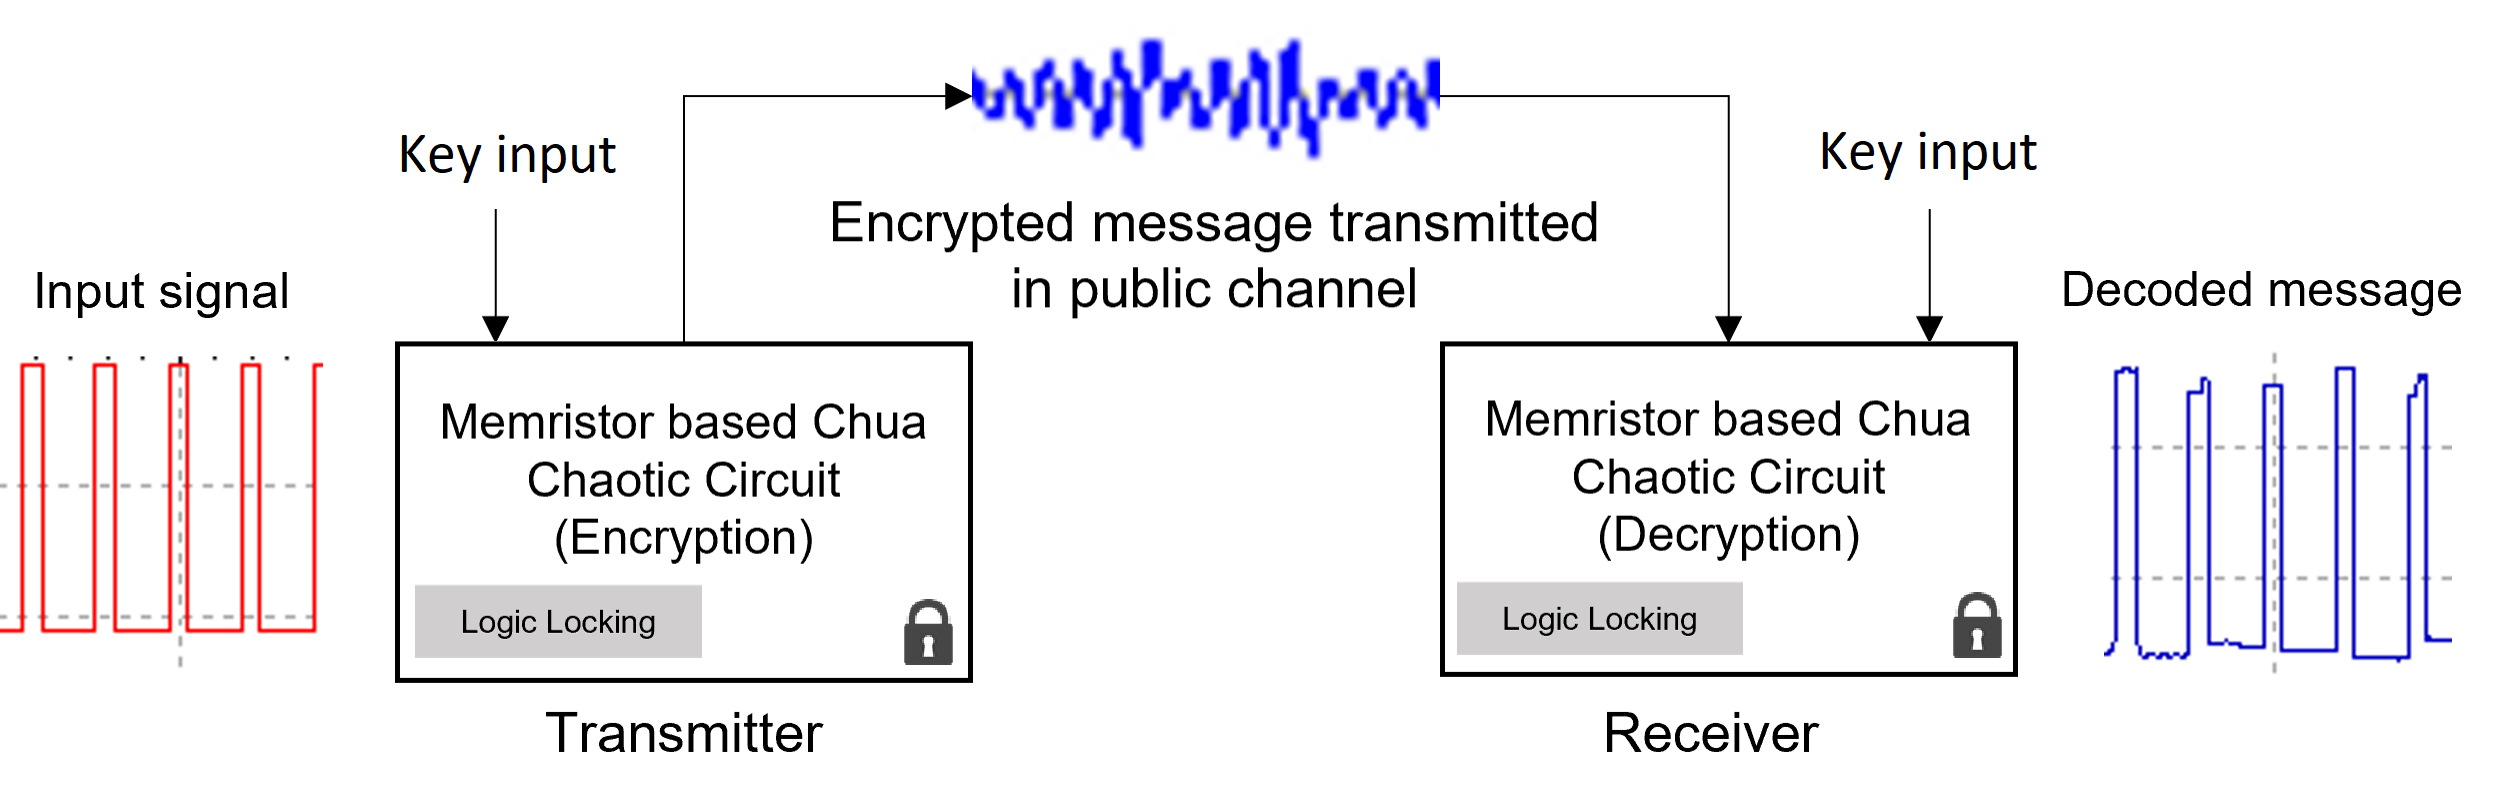
\includegraphics[width = 1\linewidth]{figs/Fig1introductionV2.png}
    \caption{Logic-locked memristor-based Chua's chaotic system}
    \label{fig:Logic-locked}
\end{figure}

The remainder of this paper is organized as follows. First, a memristor model is designed in the LTSpice Simulator in Section II. The implementation of memristor-based Chua's chaotic circuit and mathematical simulation of the circuit using MATLAB Simulink is shown in Section III. Further, in Section IV, a secure transceiver is designed using a logic-locked memristor-based chaotic circuit. Section V shows the experimental results, and the paper concludes with Section VI.

\section*{Preliminaries}\label{prelim}


\subsection*{Attack Model}
In this paper, we consider two attack models:
\begin{itemize}
\item Eavesdropper: The attacker passively listens to transceivers' communications to gain access to transmitted information. It is a privacy threat, and in our case, the goal of the eavesdropper is to find out private information about the user who uses implementable and wearable devices. 
\item Untrusted foundry: The attacker resides in the foundry and can duplicate the transceivers. It is a security threat, and in our case, the goal of the untrusted foundry is either to make a financial profit by selling unauthorized devices to the gray market or to synchronize with authorized implementable and wearable devices to send malicious actions. 
\end{itemize}
Please note that we consider that testing will be done in-house, and thus the test/verification engineer is trusted.


\subsection*{Memristor Model}
A memristor is a two-terminal electrical component relating electric charge and magnetic flux linkage. It can be viewed as a form of non-volatile memory that is based on resistance switching, which increases the flow of current in one direction and decreases the flow of current in the opposite direction. There are primarily three types of memristor model: linear, non-linear, and threshold adaptive. To add non-linearity at the boundaries, window functions are used \cite{Joglekar-Memristor, 5934403}. We use HP Memristor Model with non-linear dopant drift for transient analysis as it offers results which are in good agreement with a part of the hitherto published experiments. A detailed implementation of the model can be found in \cite{biolek2009spice}. The total resistance of the memristor R\textsubscript{MEM} is given by the below equations.
\begin{equation}
R\textsubscript{MEM}(x) = R\textsubscript{ON} (x) + R\textsubscript{OFF} (1-x),
\end{equation}

\begin{equation}
x = \frac{w}{D}\in(0,1)     
\end{equation}

Fig. \ref{fig:memristor} shows the component model of the memristor on LTSpice XVII(x64) (17.0.34.0).
\begin{figure}[ht]
    \centering
    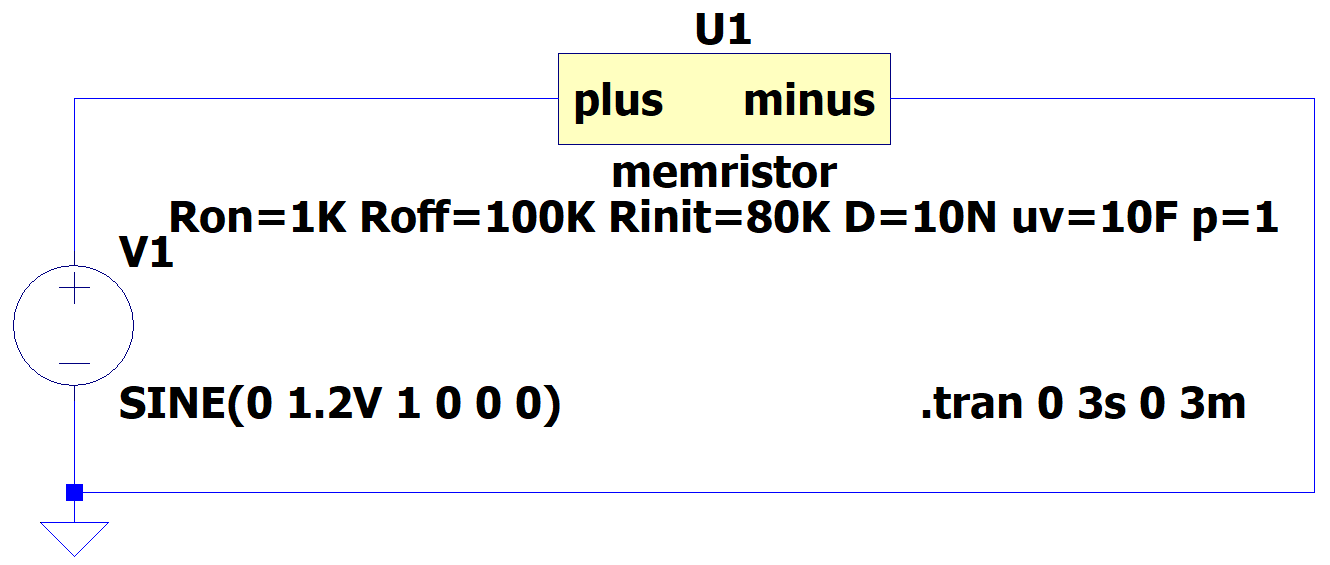
\includegraphics[width = 0.6\linewidth]{figs/Fig2memristor_model.PNG}
    \caption{Memristor component model}
    \label{fig:memristor}
\end{figure}

\subsection*{Chua's Chaotic Circuit}
Chaos can be defined as the unpredictability of a deterministic system that is highly dependent on its initial conditions. In \cite{hedayatipour2021comprehensive} different modes of chaotic equations such as Lorenz \cite{246163}, R$\ddot{o}$ssler \cite{7910544}, Chua \cite{Chua1995} and Lü \cite{ electronics10030359} have been compared for various performance metrics.

 Chua's circuit generates a chaotic behavior which is identified by a double scroll attractor or a spiral attractor. There are a few criteria for a circuit to exhibit chaotic behavior which include one or more non-linear elements, one or more resistors operating locally at the same time, and three or more energy storage elements.


 \begin{figure}[!t]
    \centering
    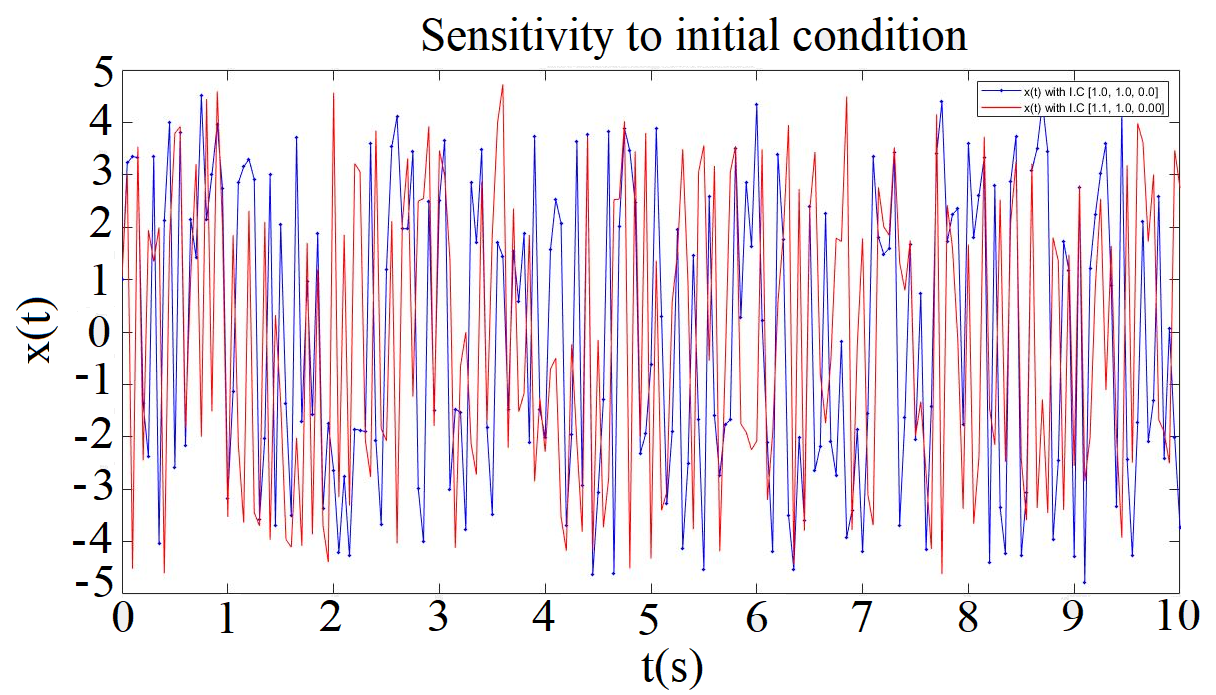
\includegraphics[width = 0.7\linewidth]{figs/Fig3Chuas_sensitivity.PNG}
    \caption{The plot of sensitivity to initial conditions of Chaos for Chua's circuit}
    \label{fig:incchua}
\end{figure}

By varying the value of one of the parameters from 1.0 to 1.1, the trajectories of x(t) are extremely
different as depicted by Fig. \ref{fig:incchua}. Thus, the Chua's circuit is the most sensitive of conventional chaotic circuits. %(Lorenz, Lü, R$\ddot{o}$ssler’s and Chua's Chaotic Equations ).
Most importantly, the Chua's circuit is one of the most basic durable experimental proofs of chaos that can be readily implemented in a variety of ways \cite{fortuna2009chua}, and provides the best performance trade-off among the others. %“one of the simplest robust experimental proof of chaos and can be easily implemented in different ways” \cite{fortuna2009chua}. 

As presented in Fig. \ref{fig:ltspice1}, two different design for Chua's chaotic equations are implemented to study the behaviour. Fig. \ref{fig:ltspice1} (a) demonstrate the design with inductor (L) valued 28mH and Fig. \ref{fig:ltspice1} (b) represents the design with the reduced inductance using the additional non-inverting amplifiers. The inductance of the circuit on the left C2 in Fig. \ref{fig:ltspice1} (b) can be calculated as below. 
    \begin{figure}[!t]
        \centering
        \subfloat[\centering ]{{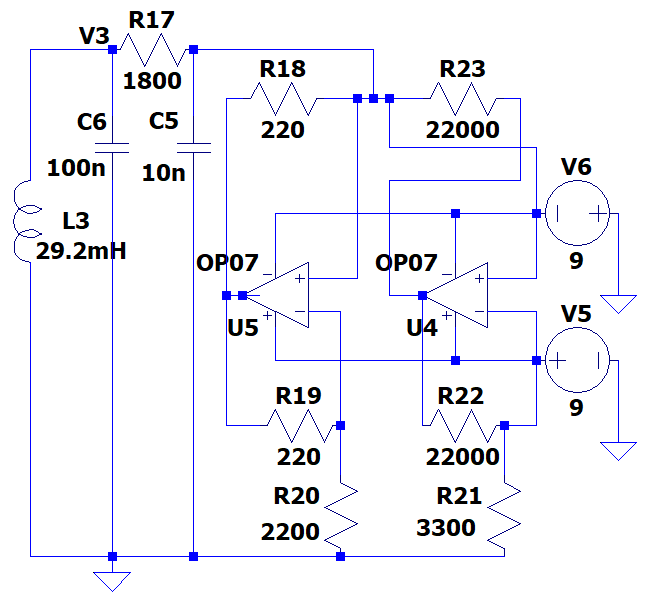
\includegraphics[scale=0.29]{figs/Fig4ach3_Chua's1st_design.PNG} }}%
        \qquad
        \subfloat[\centering ]{{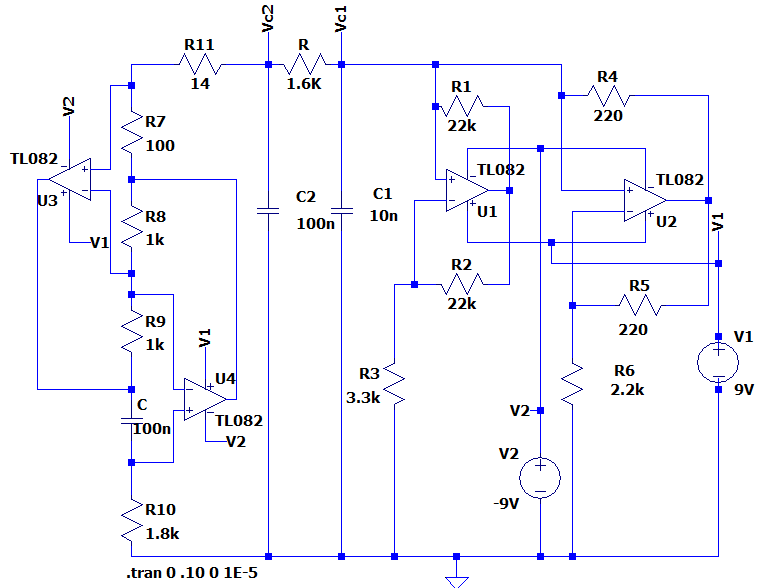
\includegraphics[scale=0.29]{figs/Fig4bch3_Chua's2nd_design.PNG} }}%
        \qquad
        \subfloat[\centering ]{{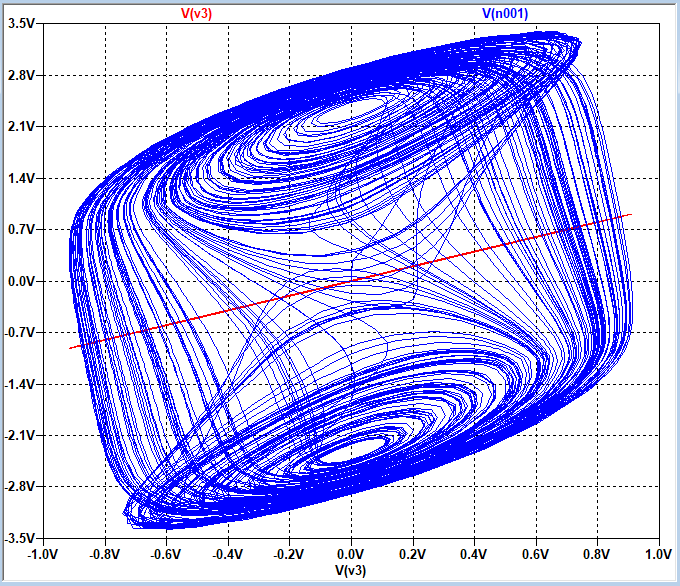
\includegraphics[height=5cm, width=5cm]{figs/Fig4cch3_Chua's1st_sim.PNG} }}%
        \qquad
        \subfloat[\centering ]{{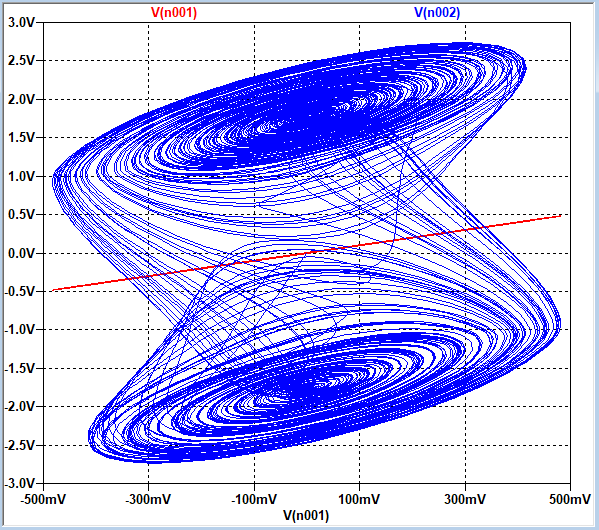
\includegraphics[height=5cm, width=5cm]{figs/Fig4dch3_Chua's2nd_sim.PNG} }}%
        \vspace{2pt}
        \caption {LTSpice design of Chau's chaos (a) with Inductor (L), (b) without Inductor (L). The attractor (c) corresponds to design in (a), and (d) corresponds to design in (b).}
        \label{fig:ltspice1}%
    \end{figure}
   % \vspace{-0.5cm}
%\[\centerline{L = (R7 * R9 * R10 * C) / R8 }  \]

\begin{equation*}
L = \frac{R7 \times R9 \times R10 \times C}{R8}    
\end{equation*}

The simulation of these LTSpice designs is shown in Fig. \ref{fig:ltspice1} (c) and (d) for designs in (a) and (b) respectively, generating Chua's attractor shape. However, the fine distinction can be observed even though they both develop Chua's attractor. The basic building block of these designs is non-inverting Operational Amplifier (Op-Amp).

In communication when the signal is discussed, it always important to pay attention to the noise component involved within the signal. Signal to Noise Ration (SNR) is the ratio of signal power compared to all other electrical signals, which can be identified as noise. SNR can be calculated by the mean of the signal divided by the standard deviation. SNR provides very critical information about the usability of the signal. Lower SNR tend to introduce the more Gaussian noise, as signal becomes unusable. This is also called `noise floor’. During the analysis of the chaotic equations, it is observed that the chaotic signal of Chua has the SNR near to 10 dB that makes signal more prone to noise and jitter attacks. Fig. \ref{fig:SNR} illustrates the SNR plot of signal X from Chua’s equation. The signal with SNR near to 10 dB can be identified as noise and the signal becomes unusable. The characteristic of these
chaotic equations is that it generates a signal as similar characteristic as noise signal even with
a message decoded in it. Thus, when transmitted through public channels these signals are just noise. Chua attains more chaos with parameter sensitivity, that symbolizes
the robustness of the chaotic equations to the static noise and eliminates possibilities of data loss.

\begin{figure}[!t]
    \centering
    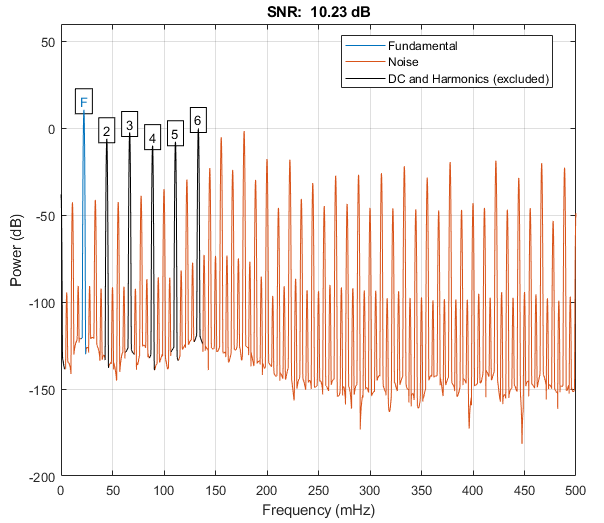
\includegraphics[width = 0.6\linewidth]{figs/Fig5SNR_chuaX.PNG}
    \caption{Signal to Noise Ratio (SNR) for Chua’s signal X}
    \label{fig:SNR}
\end{figure}


\section*{Memristor-based Chua's Chaotic Circuit}

The implementation of memristor-based Chua's chaotic circuit is described in \cite{muthuswamy2010implementing} and the same chaotic circuit is implemented using two memristors in \cite{bao2017two}. In this work, to increase the key space, we have used more than two memristors in Chua's chaotic circuit. 

\subsection*{Circuit Design in LTSpice}
Usually, for the non-linear element, a Chua's diode is utilized; however, we have used a memristor instead of a Chua's diode and also replaced a few other resistors with memristors as shown in Fig. \ref{fig:3}.

\begin{figure}[!t]
    \centering
    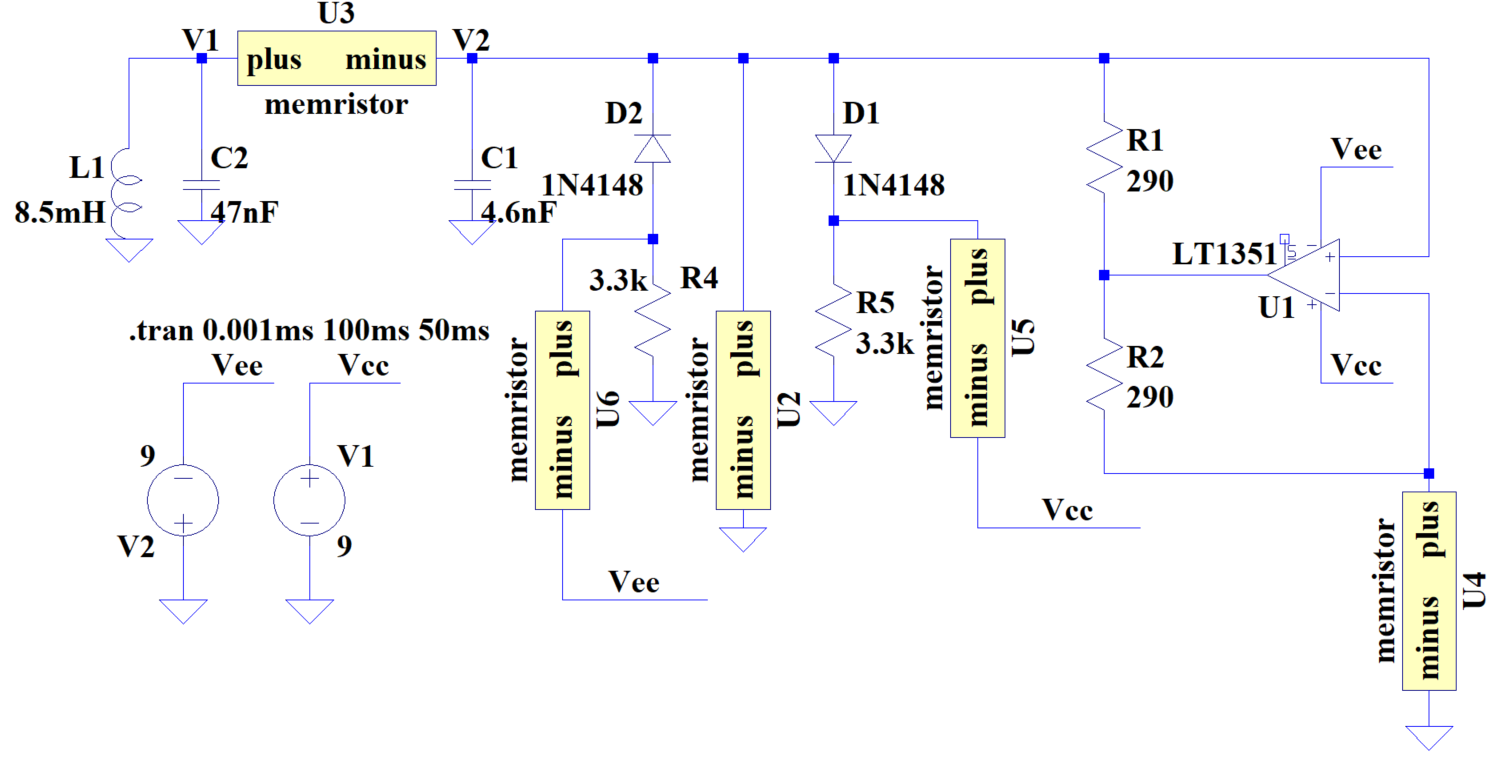
\includegraphics[width = 0.9\linewidth]{figs/Fig6chua_memristor_LTSpice.PNG}
    \caption{Implementation of memristor-based Chua's chaotic circuit}
    \label{fig:3}
\end{figure}

\begin{figure}[!t]
    \centering
    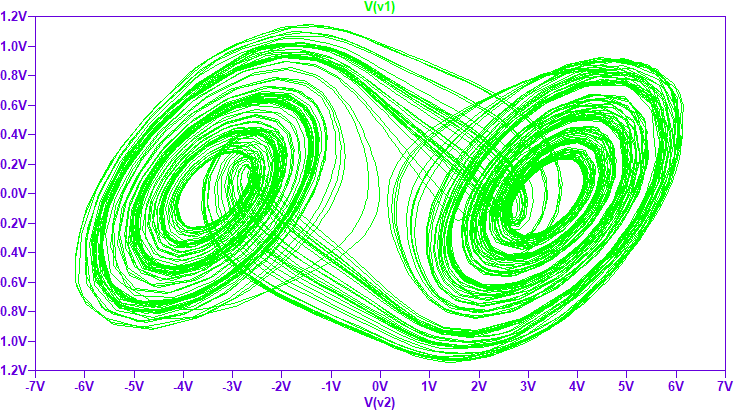
\includegraphics[width = 0.5\linewidth]{figs/Fig7double_scroll_attractor.PNG}
    \caption{Double scroll attractor for memristor U3 in Chua's chaotic circuit with values R$_{on}$=0.8K R$_{off}$=1.65K R$_{init}$=1.65K D=70N uv=10F p=1}
    \label{fig:4}
\end{figure}

\begin{figure*}[]
    \centering
    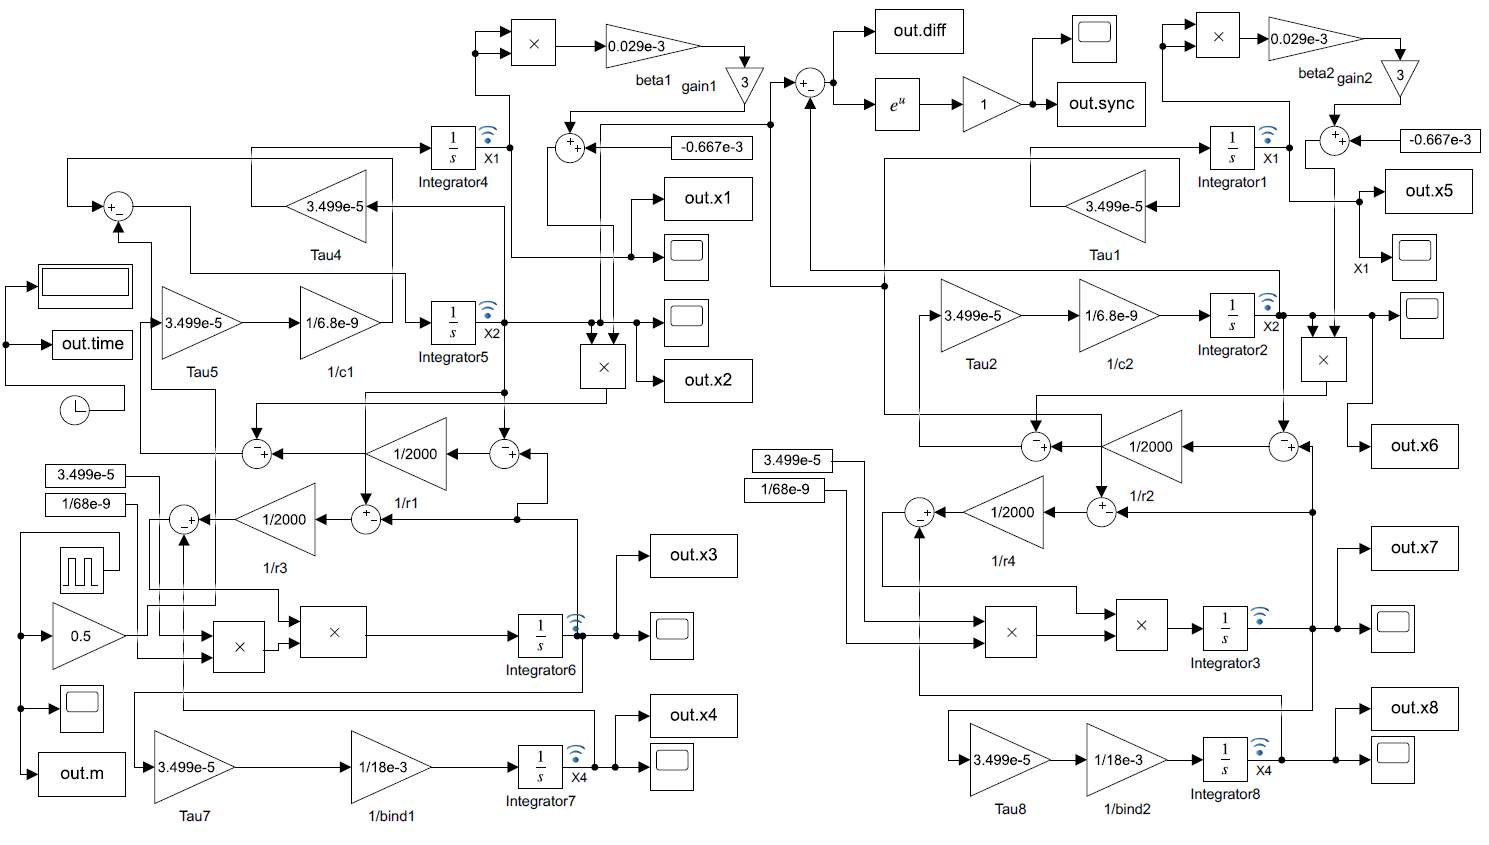
\includegraphics[width = 1\linewidth]{figs/Fig8output_simulink.PNG}
    \caption{Simulation of memristor-based Chua's chaotic circuit in MATLAB Simulink}
     \label{fig:5}
\end{figure*}

The chaotic behavior of our designed circuit is shown in Fig. \ref{fig:4} as a double scroll attractor by plotting I-V characteristics for memristor U3 in the circuit. The values of the other memristors are tuned in a range such that they satisfy the chaotic equations to exhibit chaotic behavior.


\subsection*{Mathematical Model in MATLAB Simulink}
Most of the researchers have focused on designing a system to reliably transmit the information from the sender to receiver \cite{guo2022novel} by making improvement in the way chaotic circuit is designed. For example, \cite{yang2014exponential} studies the synchronization of chaotic circuit for discontinuous chaotic systems, and \cite{9630142} uses time-scaling chaotic shift keying encryption for wireless systems. Based on the introduction of a non-linear element, i.e., memristor in the Chua's chaotic circuit, we derived the following system of equation by applying Kirchhoff Law around the loop. Fig. \ref{fig:5} shows the simulation of chaotic communication using memristor-based Chua's circuit in MATLAB Simulink.
 
\begin{equation}
\frac{d\Phi}{dt} = v\textsubscript{1}
\end{equation}

\begin{equation}
\frac{dv\textsubscript{1}(t)}{dt} = \frac{1}{C\textsubscript{1}} \left( \frac{v\textsubscript{2}(t) - v\textsubscript{2}(t)} {R} - i\textsubscript{L}(t) \right)
\end{equation}

\begin{equation}
\frac{dv\textsubscript{2}(t)}{dt} = \frac{1}{C\textsubscript{2}} \left( \frac{v\textsubscript{2}(t) - v\textsubscript{2}(t)} {R} - i\textsubscript{L}(t) \right)
\end{equation}

\begin{equation}
\frac{di\textsubscript{L}(t)}{dt} = \frac{v\textsubscript{2}(t)}{L} 
\end{equation}

The Runge–Kutta method was used, using the ode45 function, with a tolerance of 1x10-9, with a sample step of 0.01 and simulating 500 seconds. Here are the initial values used in Simulink: 
r=2000.0; 
c1=6.8e-9;	
c2=68.0e-9;	
bind=18.0e-3;
alpha = -0.667D-03;
beta=0.029D-03; 
tau=3.499e-05;
cn1=tau/c1r;
cn2=tau/c2*r; 
cn3=tau/bind;
tspan = 0:0.01:500;
x1 = 0.1; 
x2 = -0.2; 
x3 = -0.003;
x4 = 0.05;

Fig. \ref{fig:6} depicts the comparison of the input signal in red and the decoded message in blue. This can be further calibrated to obtain the accurate decoded message.  

\begin{figure}[!b]
    \centering
    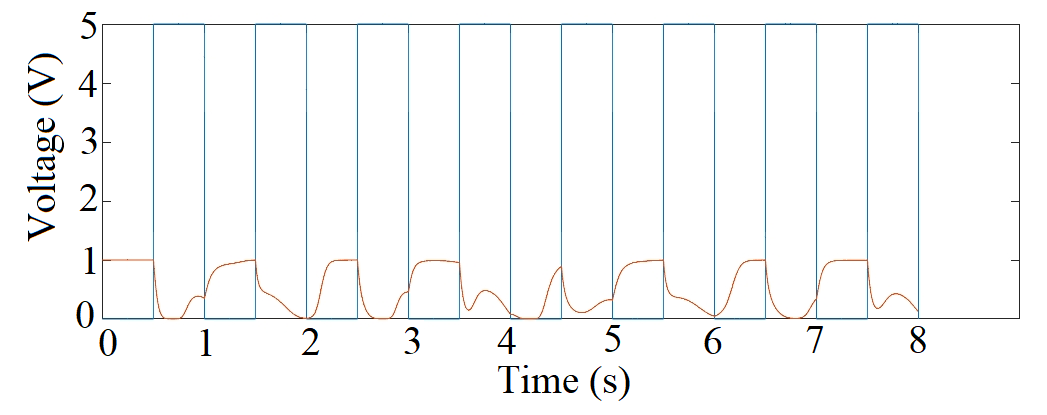
\includegraphics[width = 0.8\linewidth]{figs/Fig9syncronization.PNG}
    \caption{Comparison of input message and decoded message}
    \label{fig:6}
\end{figure}

\section*{Logic-Locked Secure Chaotic Transceivers}



With the existing research, much of the work has been done to design and improve the reliability of data transfer against eavesdroppers using chaotic communication; however, we see a gap in the security of the transceiver design itself. There can be a risk-sensitive scenario where an attacker from an untrusted foundry recreates the transceivers. To overcome this problem, we have the design goal of securing the transceivers by taking inspiration from the properties of logic locking in digital circuits. The circuit can be locked, and the locked version can be sent to the foundry for manufacturing; once the prototyped locked circuit has been returned to the design house, only the authorized users can unlock the original functionality by plugging in the secret key {\color{red}(i.e, programming the memristors based on their predefined continues values.)}

While state-of-the-art logic locking methods \cite{Koushanfar-LL,limaye2021fortifying,9427060} have focused on designing key-controlled logic gates targeted to secure purely digital circuits or designing digital keys for mixed-signal circuits \cite{8715043}, the main idea in our work is to lock the mixed-signal circuit using the analog memristors, and as we can tune the resistance value of the memristors, these continuous values can act like an analog secret key. Please note that, structurally, all the memristors used are indistinguishable, and the inside foundry attacker cannot find the value of their resistance by analyzing the circuit layout. While the key value in digital logic locking needs to be inserted into a so-called tamper-proof memory that itself may be the point of attack, here the key value is embedded into the circuit and programmed after the manufacturing.

Another part of secure and reliable communication is the design of chaotic circuits. The ``key'' values (i.e., memristors' values) will be in a certain range, which will always satisfy the chaotic equations. Although this gives a hint to the attacker to at least make an estimate of the range of values and perform the attack, even then, it will be difficult to start with brute-force as there are multiple memristors in the circuit with exponentially large key space. LTSpice model of our proposed logic-locked transmitter and receiver is shown in Fig. \ref{fig:7}. The input message is a pulse signal, which is mixed with the chaotic message, and finally it will be decoded at the receiver end. A \(\beta\)-modulator is also used in the circuit, which is a variable gain circuit designed with an inverting summing amplifier and two separate inverting amplifiers, and is controlled by a switch.

\begin{figure*}[]
    \centering
    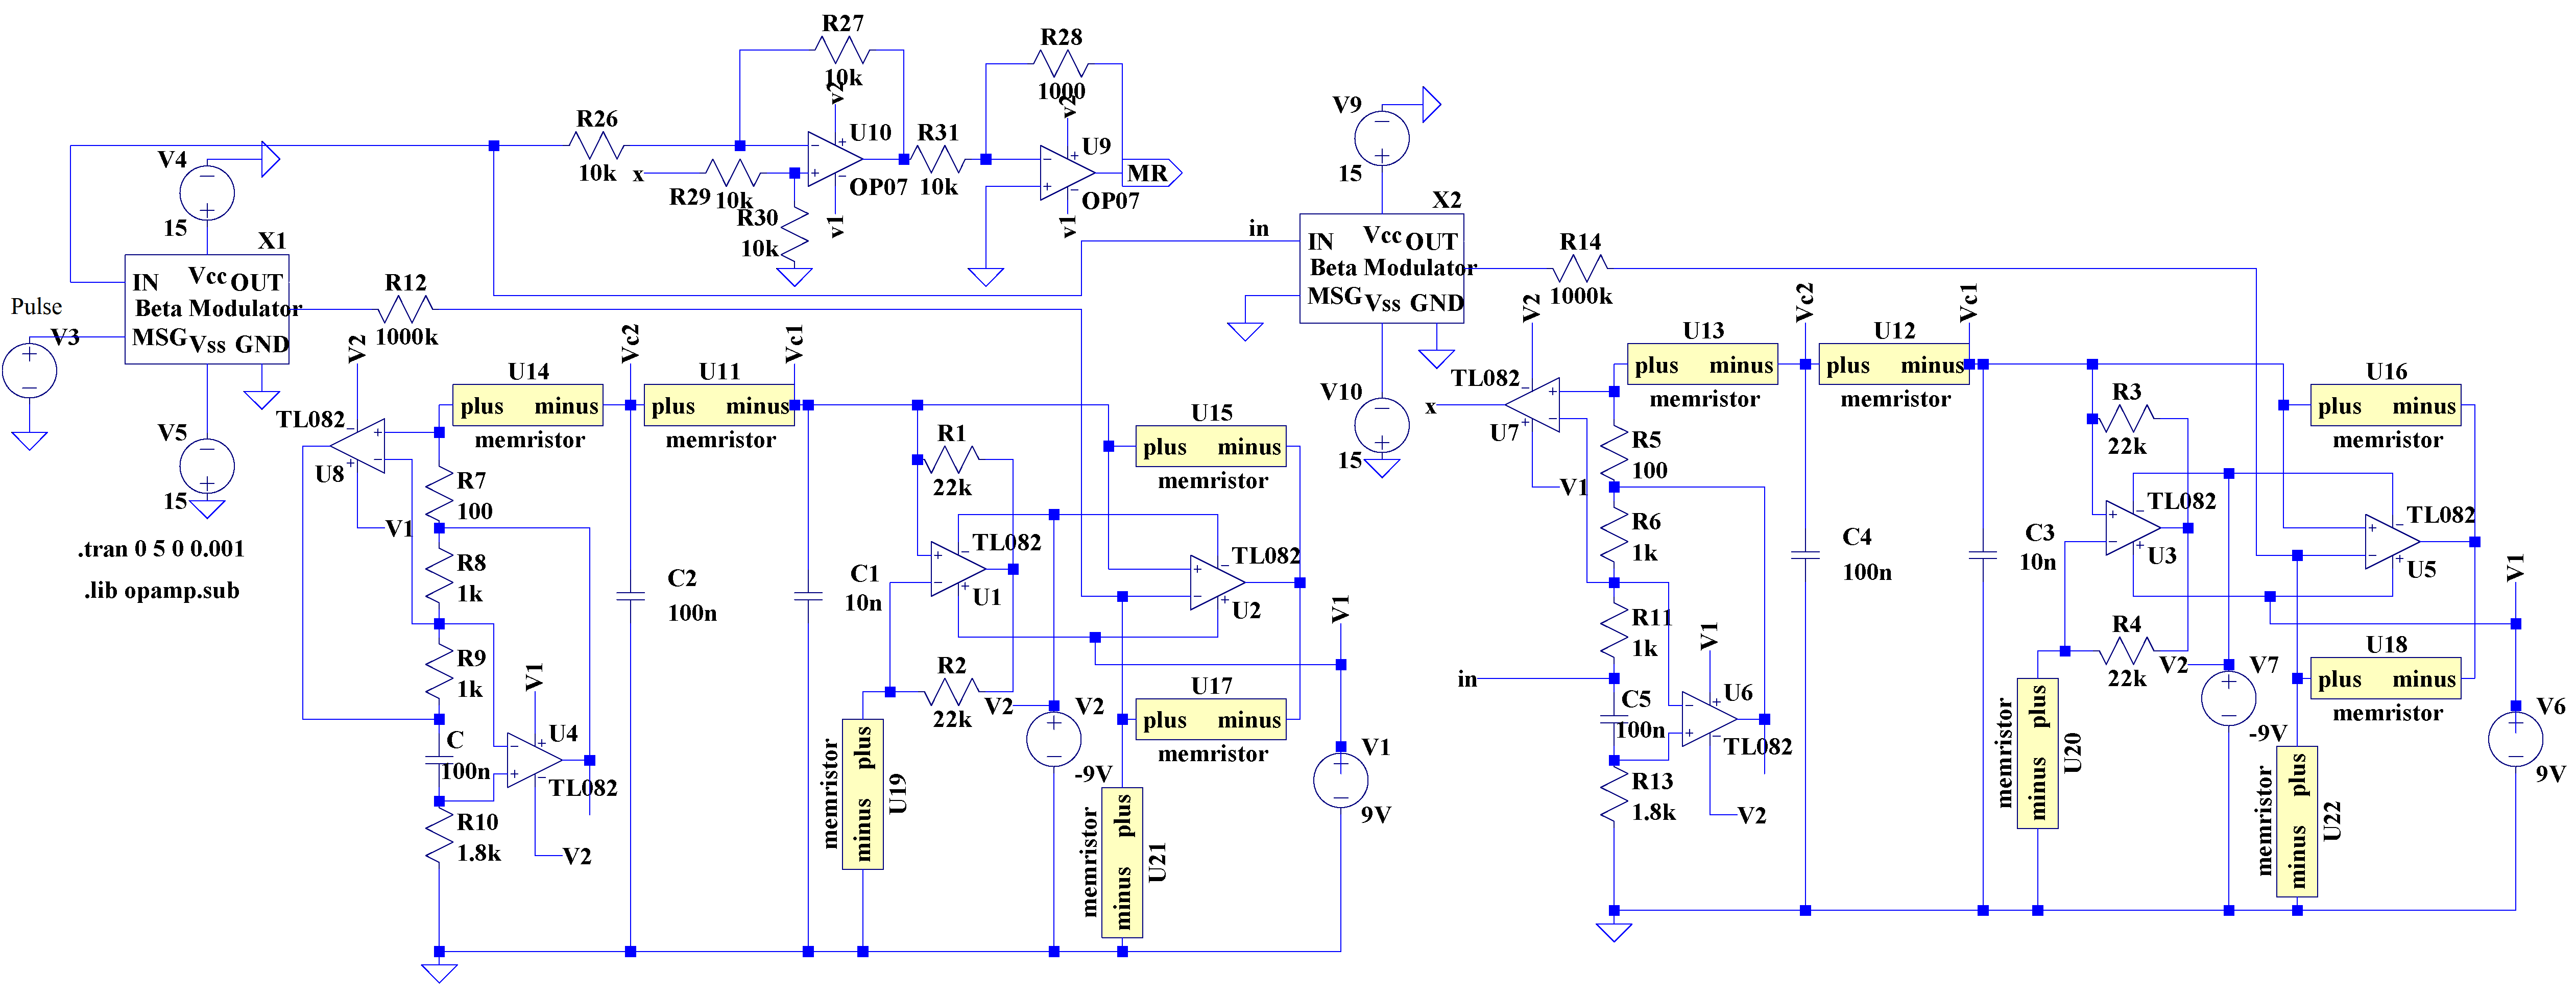
\includegraphics[width = 1\linewidth]{figs/Fig10Tx_Rx_LTSpice.PNG}
    \caption{LTSpice design of transmitter and receiver for memristor-based Chua's chaotic circuit}
     \label{fig:7}
\end{figure*}

\begin{figure}[!b]
    \centering
    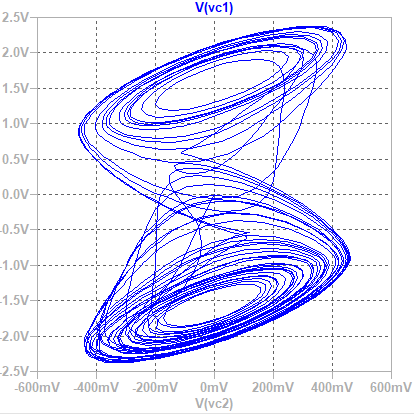
\includegraphics[width = 0.65\linewidth]{figs/Fig11double scroll attractor.PNG}
    \caption{Double scroll attractor of Chua's chaotic circuit with memristor value R\textsubscript{OFF} = 1.6K for T\textsubscript{x} (U11) and R\textsubscript{x} (U12) }
     \label{fig:8}
\end{figure}

\subsection*{Attack Analysis}
The logic locking methods designed for digital circuits with an $n$-bit key size have 2$^n$ cases with discrete values, such that R$_{i}$ $\in$ $\{0,$ 1$\}$ $\rightarrow$ 2$^n$ which cannot be broken by brute-force attack but may be challenged by the SAT-based attack \cite{7140252} that adopts a stronger attacker model by using both a locked version of the circuit and an activated transceiver bought off the market. As the SAT-based attack can handle only Boolean variables, it cannot break analog logic locking. But and advanced attack version based on satisfiability modulo theories (SMT) \cite{9000113} can be applicable here.

However, our research focuses on the use of continuous values for the keys $R\textsubscript{i}$ $\in$ $[0, R\textsubscript{max}]$ which is equivalent to the discrete form with many possibilities. Assuming we have $R\textsubscript{max}$ $=$ $m\Delta$, the above relationship can be written as $R\textsubscript{i}$ $\in$ $[0$, $\Delta$, 2$\Delta$, 3$\Delta$, ..., m$\Delta$] $\rightarrow$ m$^n$. For each memristor value, there are $m\Delta$ possibilities with $m >> n$. In comparison with the traditional method, we have m$^n$\texttt{>>}n$^n$$\texttt{>>}$2$^n$, which is double exponential.In this case, even for the SMT attack \cite{9000113}, the key size will be exponentially large, and not possible to be deciphered in polynomial time. We complement our attack analysis via experiments in Section \ref{experiments}.

\section*{Experimental results} \label{experiments}
We experimentally implemented different transceivers simulated in \cite{hedayatipour2021comprehensive} using FPGA board Nexys A7 for the system generator design of Lorenz, SprottD, and Chua as shown in Fig. \ref{fig:hwcosim2}. The parameter values, generated in XSG is taken to the MATLAB to plot them and is shown in Fig. \ref{fig:XSG}. When comparing these experimental plots with the simulation plot, it can be seen that the hardware experimental data matches the attractor shape for each equation and generates the chaos. The details of these hardware implementation is published in our recent work \cite{monani2022implementation}.

    \begin{figure}[!ht]
        \centering
        \subfloat[\centering ]{{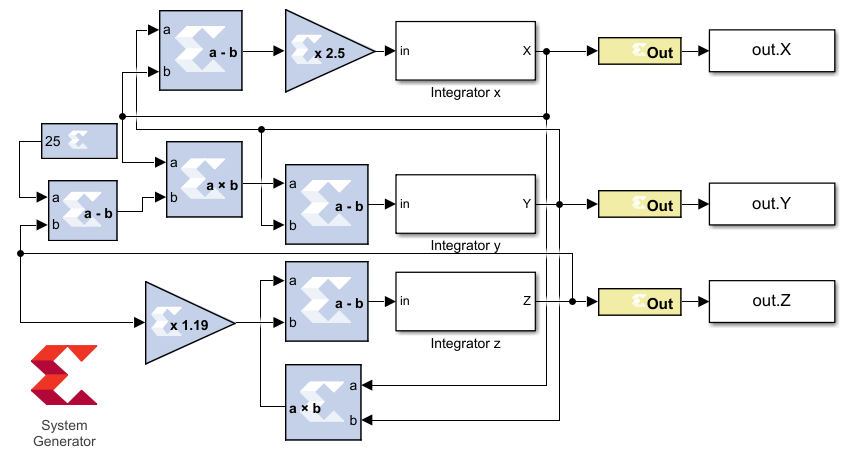
\includegraphics[height=4cm, width=7cm]{figs/Fig12aLorenz_XSG.PNG} }}%
        \qquad
        \subfloat[\centering ]{{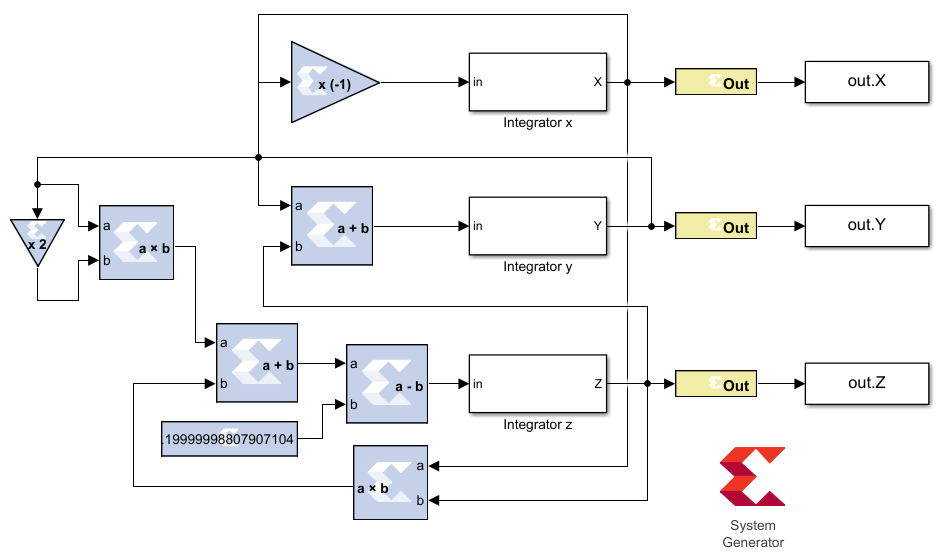
\includegraphics[height=4cm, width=7cm]{figs/Fig12bSprottD_XSG.PNG} }}%
        \qquad
        \subfloat[\centering ]{{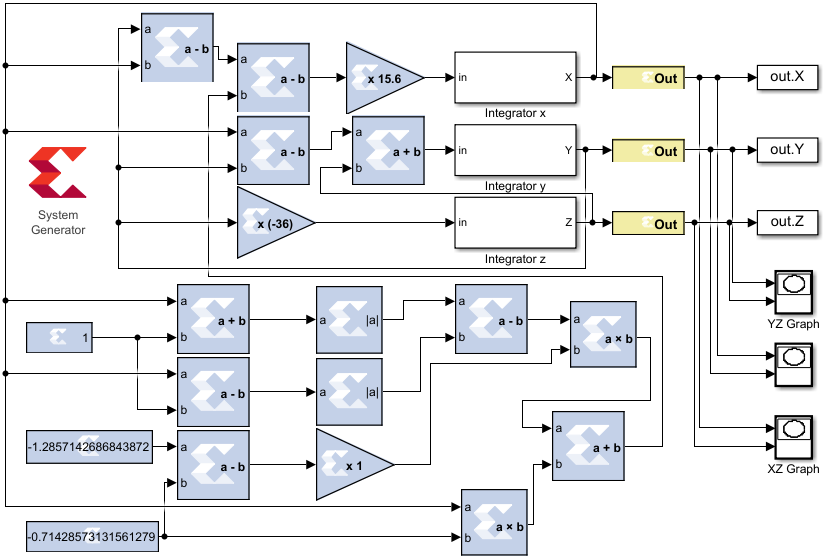
\includegraphics[scale= 0.4]{figs/Fig12cXSG_Chua.PNG} }}%
        \vspace{1pt}
        \caption{XSG Design for Transmitter of (a) Lorenz, (b) SprottD, and (c) Chua.}
        \label{fig:hwcosim2}%
    \end{figure}



        \begin{figure}[ht]
        \centering
        \subfloat[\centering ]{{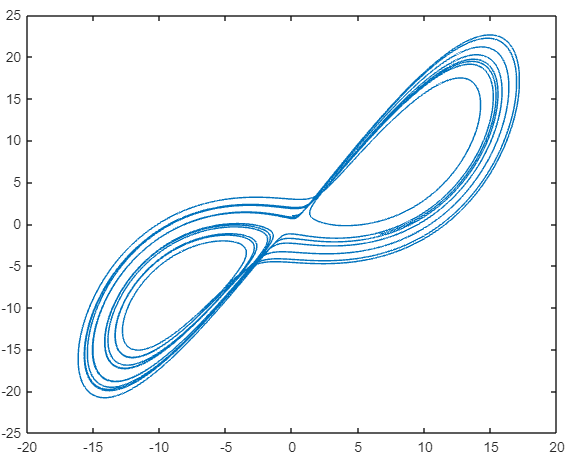
\includegraphics[height=4cm, width=4cm]{figs/Fig13aLorenz_XY_XSG.PNG} }}%
        %\qquad
        \subfloat[\centering ]{{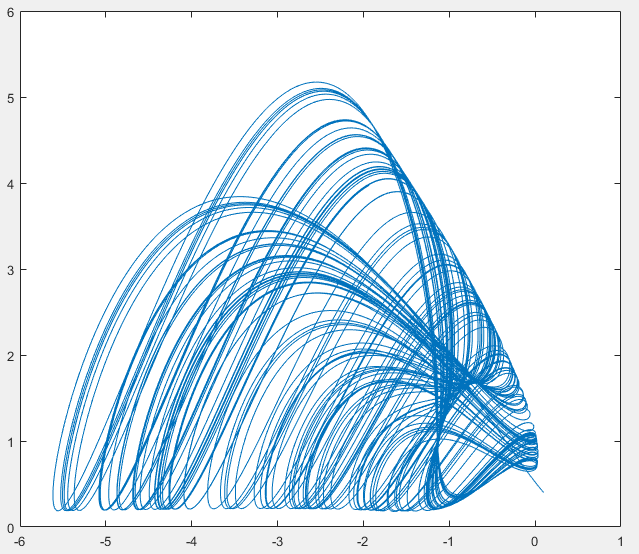
\includegraphics[height=4cm, width=4cm]{figs/Fig13bSprottD_XZ_XSG.PNG} }}%
        %\qquad \vspace{-0.2cm}
        \subfloat[\centering ]{{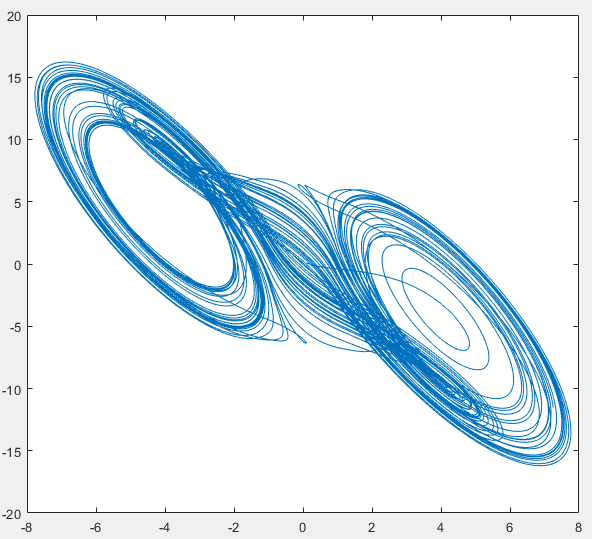
\includegraphics[height=4cm, width=4cm]{figs/Fig13cChua_XZ_XSG.PNG} }}%
       % \vspace{2pt}
        \caption{XSG hardware co-simulation plot for (a) Lorenz, (b) (SprottD), and (c) Chua.}
        \label{fig:XSG}%
    \end{figure}

The post-synthesis and the post-implementation data are represented in Table \ref{tab:resources}  for the hardware utilization. These hardware resources can be considered as Look-Up Table (LUT), Flip-Flops (FF), and Digital Signal Processors (DSP). The chart of these comparisons can also be seen in Figure \ref{fig:resource} (b).

\begin{table}[b]
	\centering
	\caption{Comparison of Resource Utilization}
	\vspace*{0.2in}
	\begin{tabular}{| c | c | c | c |c | }
		\hline
		Design & Resource & Available & Utilization & Utilization in \% \\ 
		\hline 
	Lorenz & LUT & 20800& 850 & 4.09 \\
	{} & FF & 41600& 96 & 0.23 \\
	{} & DSP & 90 & 15 & 16.67 \\
	\hline 
	SprottD & LUT & 20800& 578 & 2.78 \\
	{} & FF & 41600& 96 & 0.23 \\
    {} & DSP & 90 & 14 & 15.56 \\
    \hline
	Chua & LUT & 20800& 933 & 4.49 \\
	{} & FF & 41600& 96 & 0.23 \\
	{} & DSP & 90& 20 & 22.22 \\
		\hline
	\end{tabular}
	\label{tab:resources}
\end{table}

 \begin{figure}[t]
        \centering
        \subfloat[\centering ]{{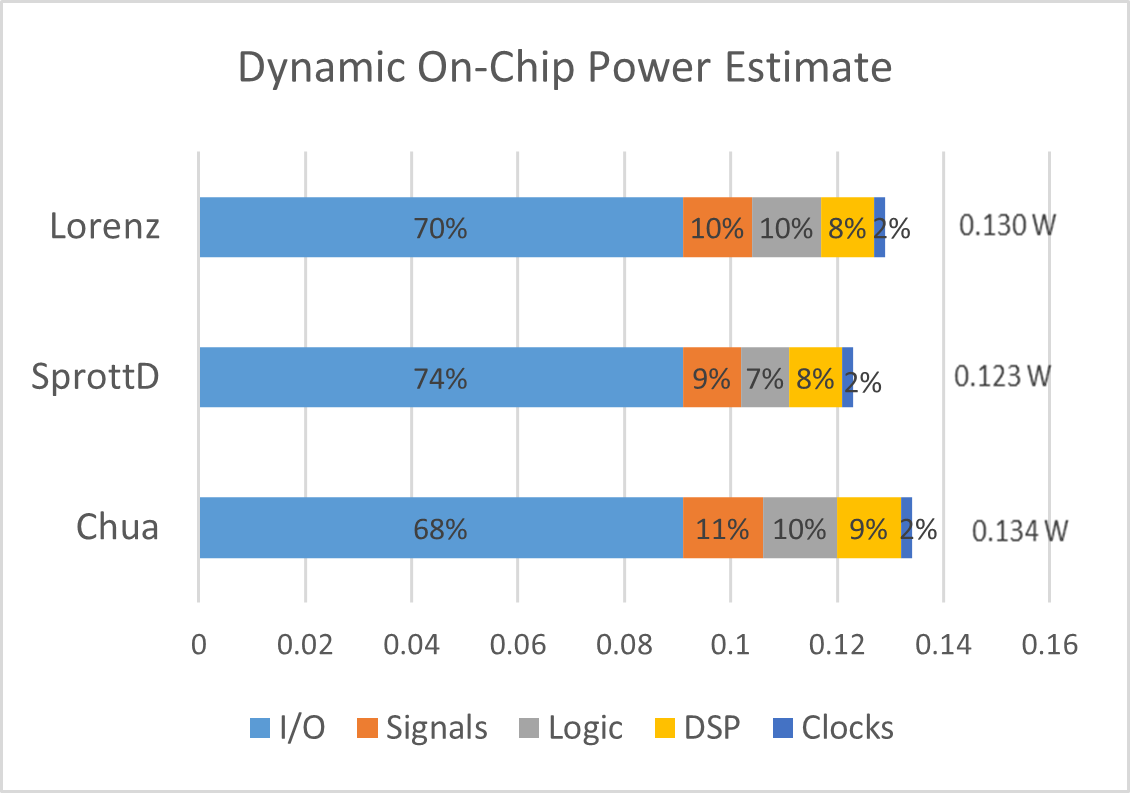
\includegraphics[height=5cm, width=7.6cm]{figs/Fig14aPower_est.png} }}%
        \qquad
        \subfloat[\centering ]{{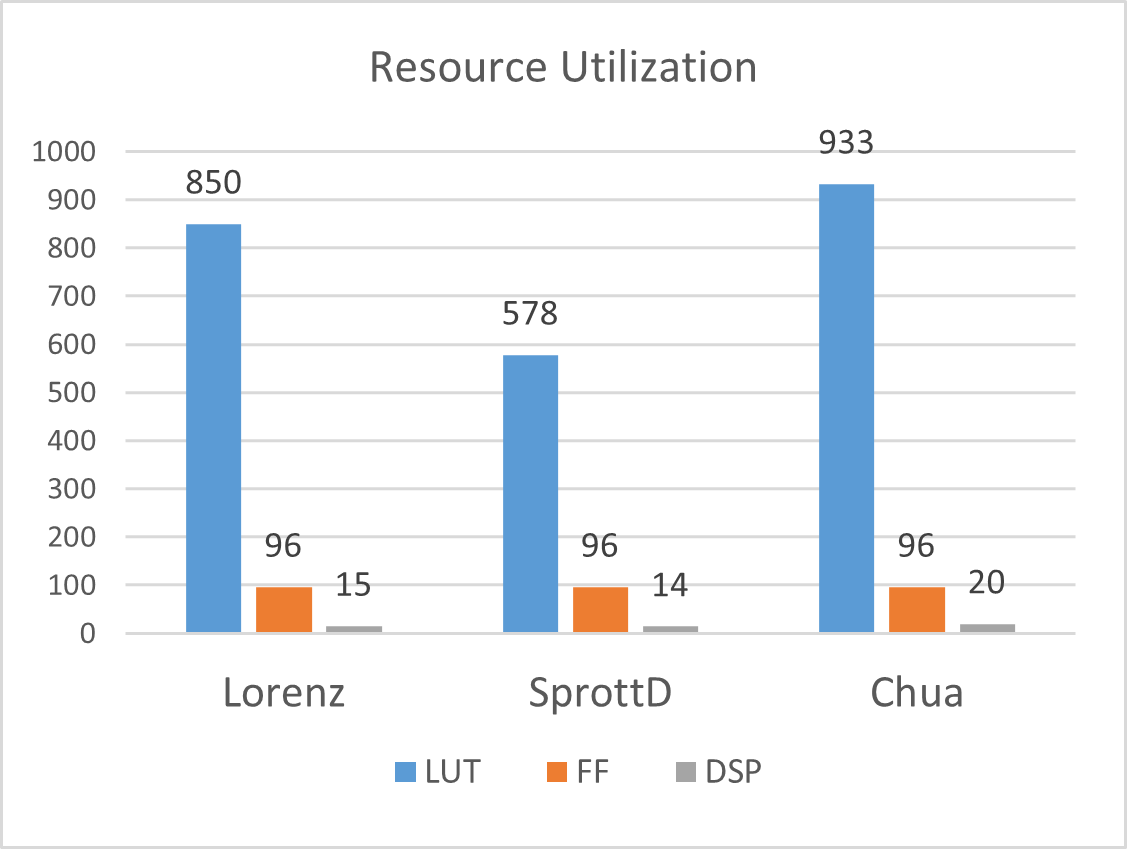
\includegraphics[height=5cm, width=7.85cm]{figs/Fig14bResource_uti.png} }}%
        \vspace{-6pt}
        \caption{Comparison of Chaotic Equation for (a) On-Chip Power Estimate, (b) Resource Utilization.}
        \label{fig:resource}%
    \end{figure}


The circuit design is shared with the untrusted foundry, and once the manufactured circuits are received, the memristor values can be tuned in-house to create a pair of transmitter and receiver that can only work together. The use of memristors secures the mechanism in that even if someone gains access to the entire circuit, the circuit will not function without the specific key inserted. On the other hand, in a situation where an eavesdropper has access to the message transmitted, he/she cannot decode the message without knowing the actual values of the memristors used in the pair of transceivers. 

Thus, for experimental validation, we will discuss two scenarios for performing chaos-based communication:
\begin{itemize}
\item \textbf{Scenario 1:} We only vary the circuit's component parameters of the transmitter, keeping the receiver's parameters constant to achieve a chaotic circuit and perform secure communication.
\item \textbf{Scenario 2:} We can have different values of the memristor component in the transmitter as well as receiver and still achieve secure communication.
\end{itemize}

\begin{figure}[!t]
    \centering
    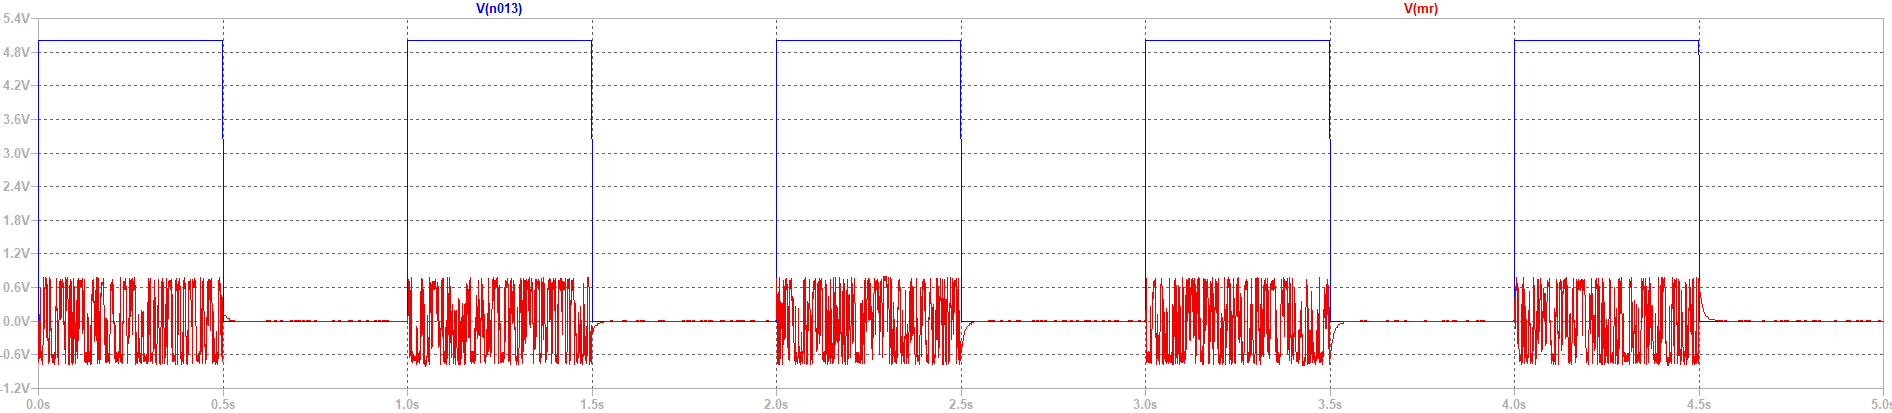
\includegraphics[width = 0.8\linewidth]{figs/Fig15U11_1_6K.PNG}
    \caption{Case 1: Original message V(n013) in blue color and decoded message V(mr) in red color}
    \label{fig:9}
\end{figure}

In the first scenario, the focus is on the chaotic circuit that can be regulated by the similar system of equations but having slightly different parameters which are in the limit of component tolerances. The second scenario focuses on the chaotic circuit with different dynamical behaviors because of the component's different parameters (parametric mismatches). Finally we also show the results of the SMT attack on our proposed transceiver in Fig. \ref{fig:7}.

\subsection*{Transmitter \& Receiver with Identical Memristors}

The two circuits, transmitter and receiver are identical, but their component's tolerance range obey the set of equations mentioned in \cite{chua1971memristor} to generate Chua's chaotic behavior. In our experiment we consider two cases and show that if the memristor's values are within the tolerance range, a secure communication is established and the encoded message is decoded successfully.  
\newline
\\
\textbf{Case 1:} Memristor parameter R\textsubscript{OFF} = 1.6K for T\textsubscript{x} (U11) and R\textsubscript{x} (U12)

The corresponding memristor values of T\textsubscript{x} and R\textsubscript{x} are set identical, but different from the suggested values mentioned in \cite{chua1971memristor}. The motive is to demonstrate large key space using memristors and establish secure and reliable chaotic communication.

\begin{center}
\small
\begin{tabular}{|c c c |} 
 \hline
 Tx & Rx & Memristor Parameters \\ [0.5ex] 
 \hline\hline
 U11 & U12 & Ron=0.8K Roff=1.6K D=70N uv=10F p=1 \\ 
 \hline
 U14 & U13 & Ron=7 Roff=14 D=70N uv=10F p=1 \\ 
 \hline
 U19 & U20 & Ron=1.65K Roff=3.3K D=70N uv=10F p=1 \\ 
 \hline
 U21 & U22 & Ron=1.1K Roff=2.2K D=70N uv=10F p=1 \\ 
 \hline
\end{tabular}
\end{center} 

The (T\textsubscript{x}, R\textsubscript{x}) memristor pairs (U11, U12), (U14, U13), (U19, U20), (U21, U22) also have a slightly different values (within the tolerance range) as mentioned in \cite{biolek2009spice} and the chaotic circuit produces a double scroll attractor as shown in Fig. \ref{fig:8}. 

Fig. \ref{fig:9} shows the decrypted signal V(mr) and is compared with the originally received signal V(n013) at the receiver end. The signal difference between them is amplified to retrieve the message signal data in order to complete the transaction. 

\textbf{Case 2:} Memristor parameter R\textsubscript{OFF} = 1.8K for T\textsubscript{x} (U11) and R\textsubscript{x} (U12)

To show that the memristor-based chaotic circuit still holds the chaotic behavior with different parameters as compared to the values used in case 1, a circuit was simulated using the below parameters of the memristors. Fig. \ref{fig:10} shows the chaotic behavior of the circuit with memristor value R\textsubscript{OFF} = 1.8K for T\textsubscript{x} (U11) and R\textsubscript{x} (U12). The comparison of input message and the decoded message is shown in Fig. \ref{fig:11}.  

\begin{center}
\small
\begin{tabular}{|c c c |} 
 \hline
 Tx & Rx & Memristor Parameters \\ [0.5ex] 
 \hline\hline
 U11 & U12 & Ron=0.9K Roff=1.8K D=70N uv=10F p=1 \\ 
 \hline
 U14 & U13 & Ron=7 Roff=13 D=70N uv=10F p=1 \\ 
 \hline
 U19 & U20 & Ron=1.65K Roff=3.2K D=70N uv=10F p=1 \\ 
 \hline
 U21 & U22 & Ron=1.1K Roff=2.19K D=70N uv=10F p=1 \\ 
 \hline
\end{tabular}
\end{center}

\begin{figure}[!b]
    \centering
    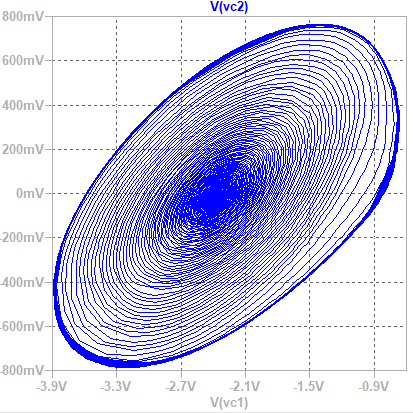
\includegraphics[width = 0.65\linewidth]{figs/Fig161_8_Spiral attractor.PNG}
    \caption{Spiral attractor of Chua's chaotic circuit with memristor value R\textsubscript{OFF} = 1.8K for T\textsubscript{x} (U11) and R\textsubscript{x} (U12)}
     \label{fig:10}
\end{figure}

\begin{figure}[!b]
    \centering
    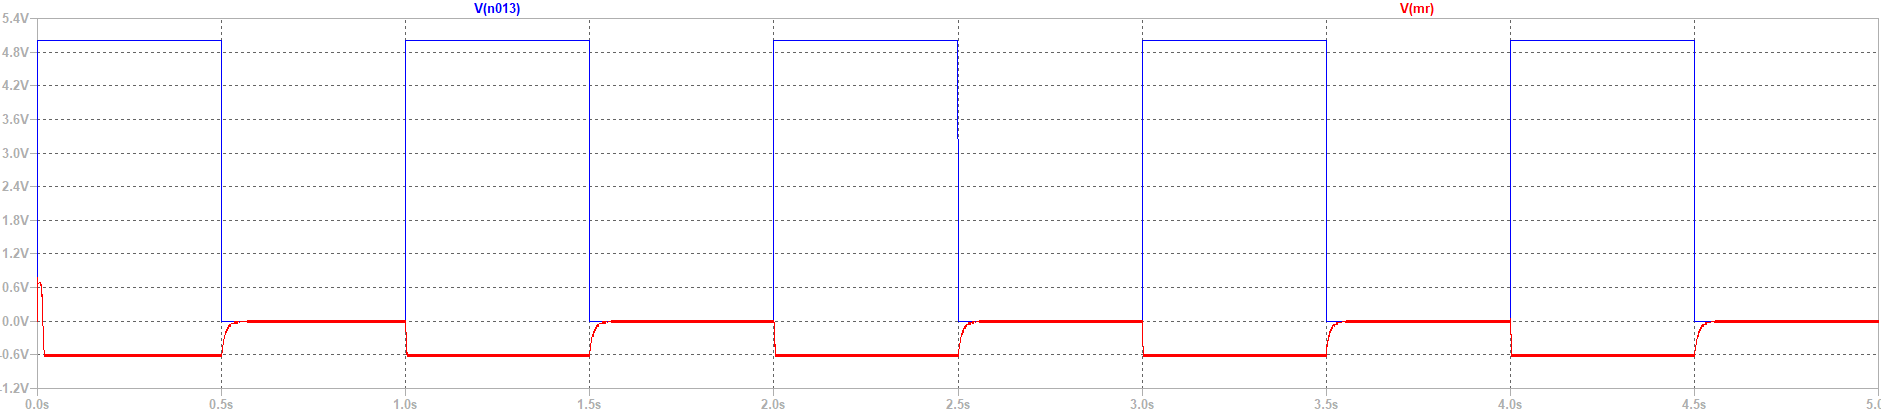
\includegraphics[width = 0.8\linewidth]{figs/Fig17U11_1_8K.PNG}
    \caption{Case 2: Original message (V(n013) in blue color and decoded message V(mr) in red color}
     \label{fig:11}
\end{figure}

Further, if the values of the memristor is changed beyond the tolerance range for which it stops exhibiting chaotic behavior, it is observed in Fig. \ref{fig:12} that the transceiver fails to decode the message.   
If we change the value of R\textsubscript{x} (U12) from Ron=0.9K Roff=1.8K D=70N uv=10F p=1 to Ron=0.9K Roff=1.79K D=70N uv=10F p=1, the message will not be decoded. So, the attacker has to be aware of all the values of the memristors present in the transmitter circuit. 

\begin{figure}[ht]
    \centering
    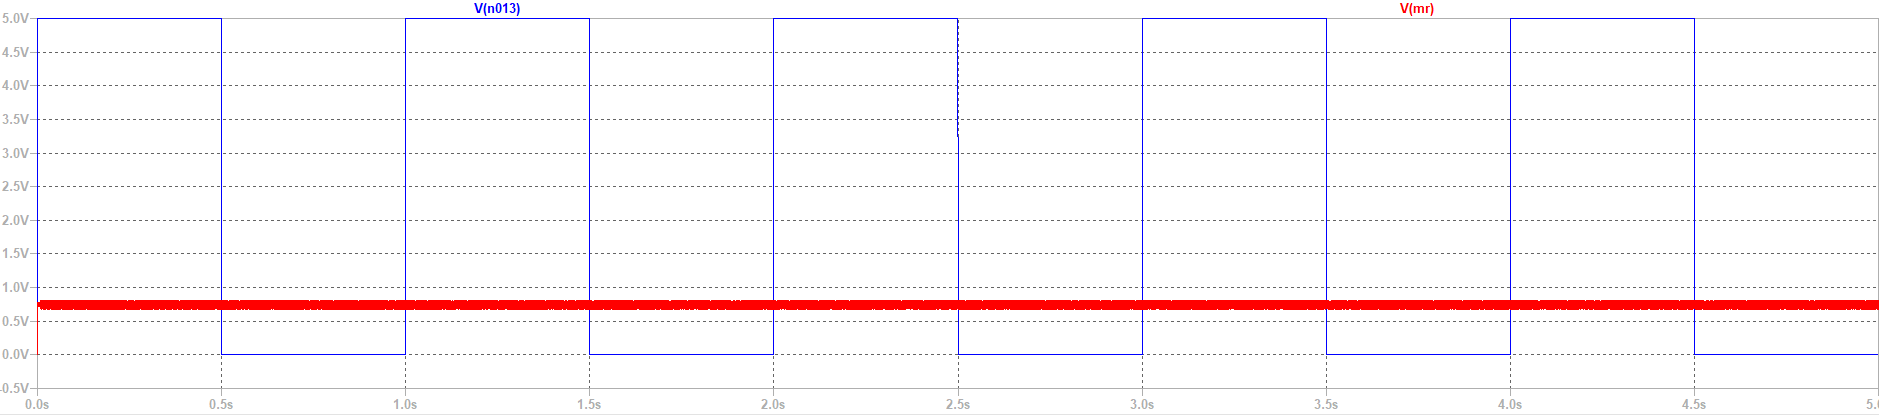
\includegraphics[width = 0.8\linewidth]{figs/Fig18U11_1_8K_no_decode.PNG}
    \caption{Message is not decoded if the memristors values are changed beyond the tolerance}
    \label{fig:12}
\end{figure}

\subsection*{Transmitter and Receiver with Non-Identical Memristors}
Second scenario is to validate if the original message is decoded at the receiver end when the Chua's chaotic circuit are non-identical, i.e., parameter mismatch. For simplicity, only one memristor value is different in transmitter and receiver, and other values of the memristor are identical. %NI Multisim 14.3 is used for designing memristor-based Chua's chaotic circuit and perform secure communication.  



\begin{figure}[!t]    
\centering
    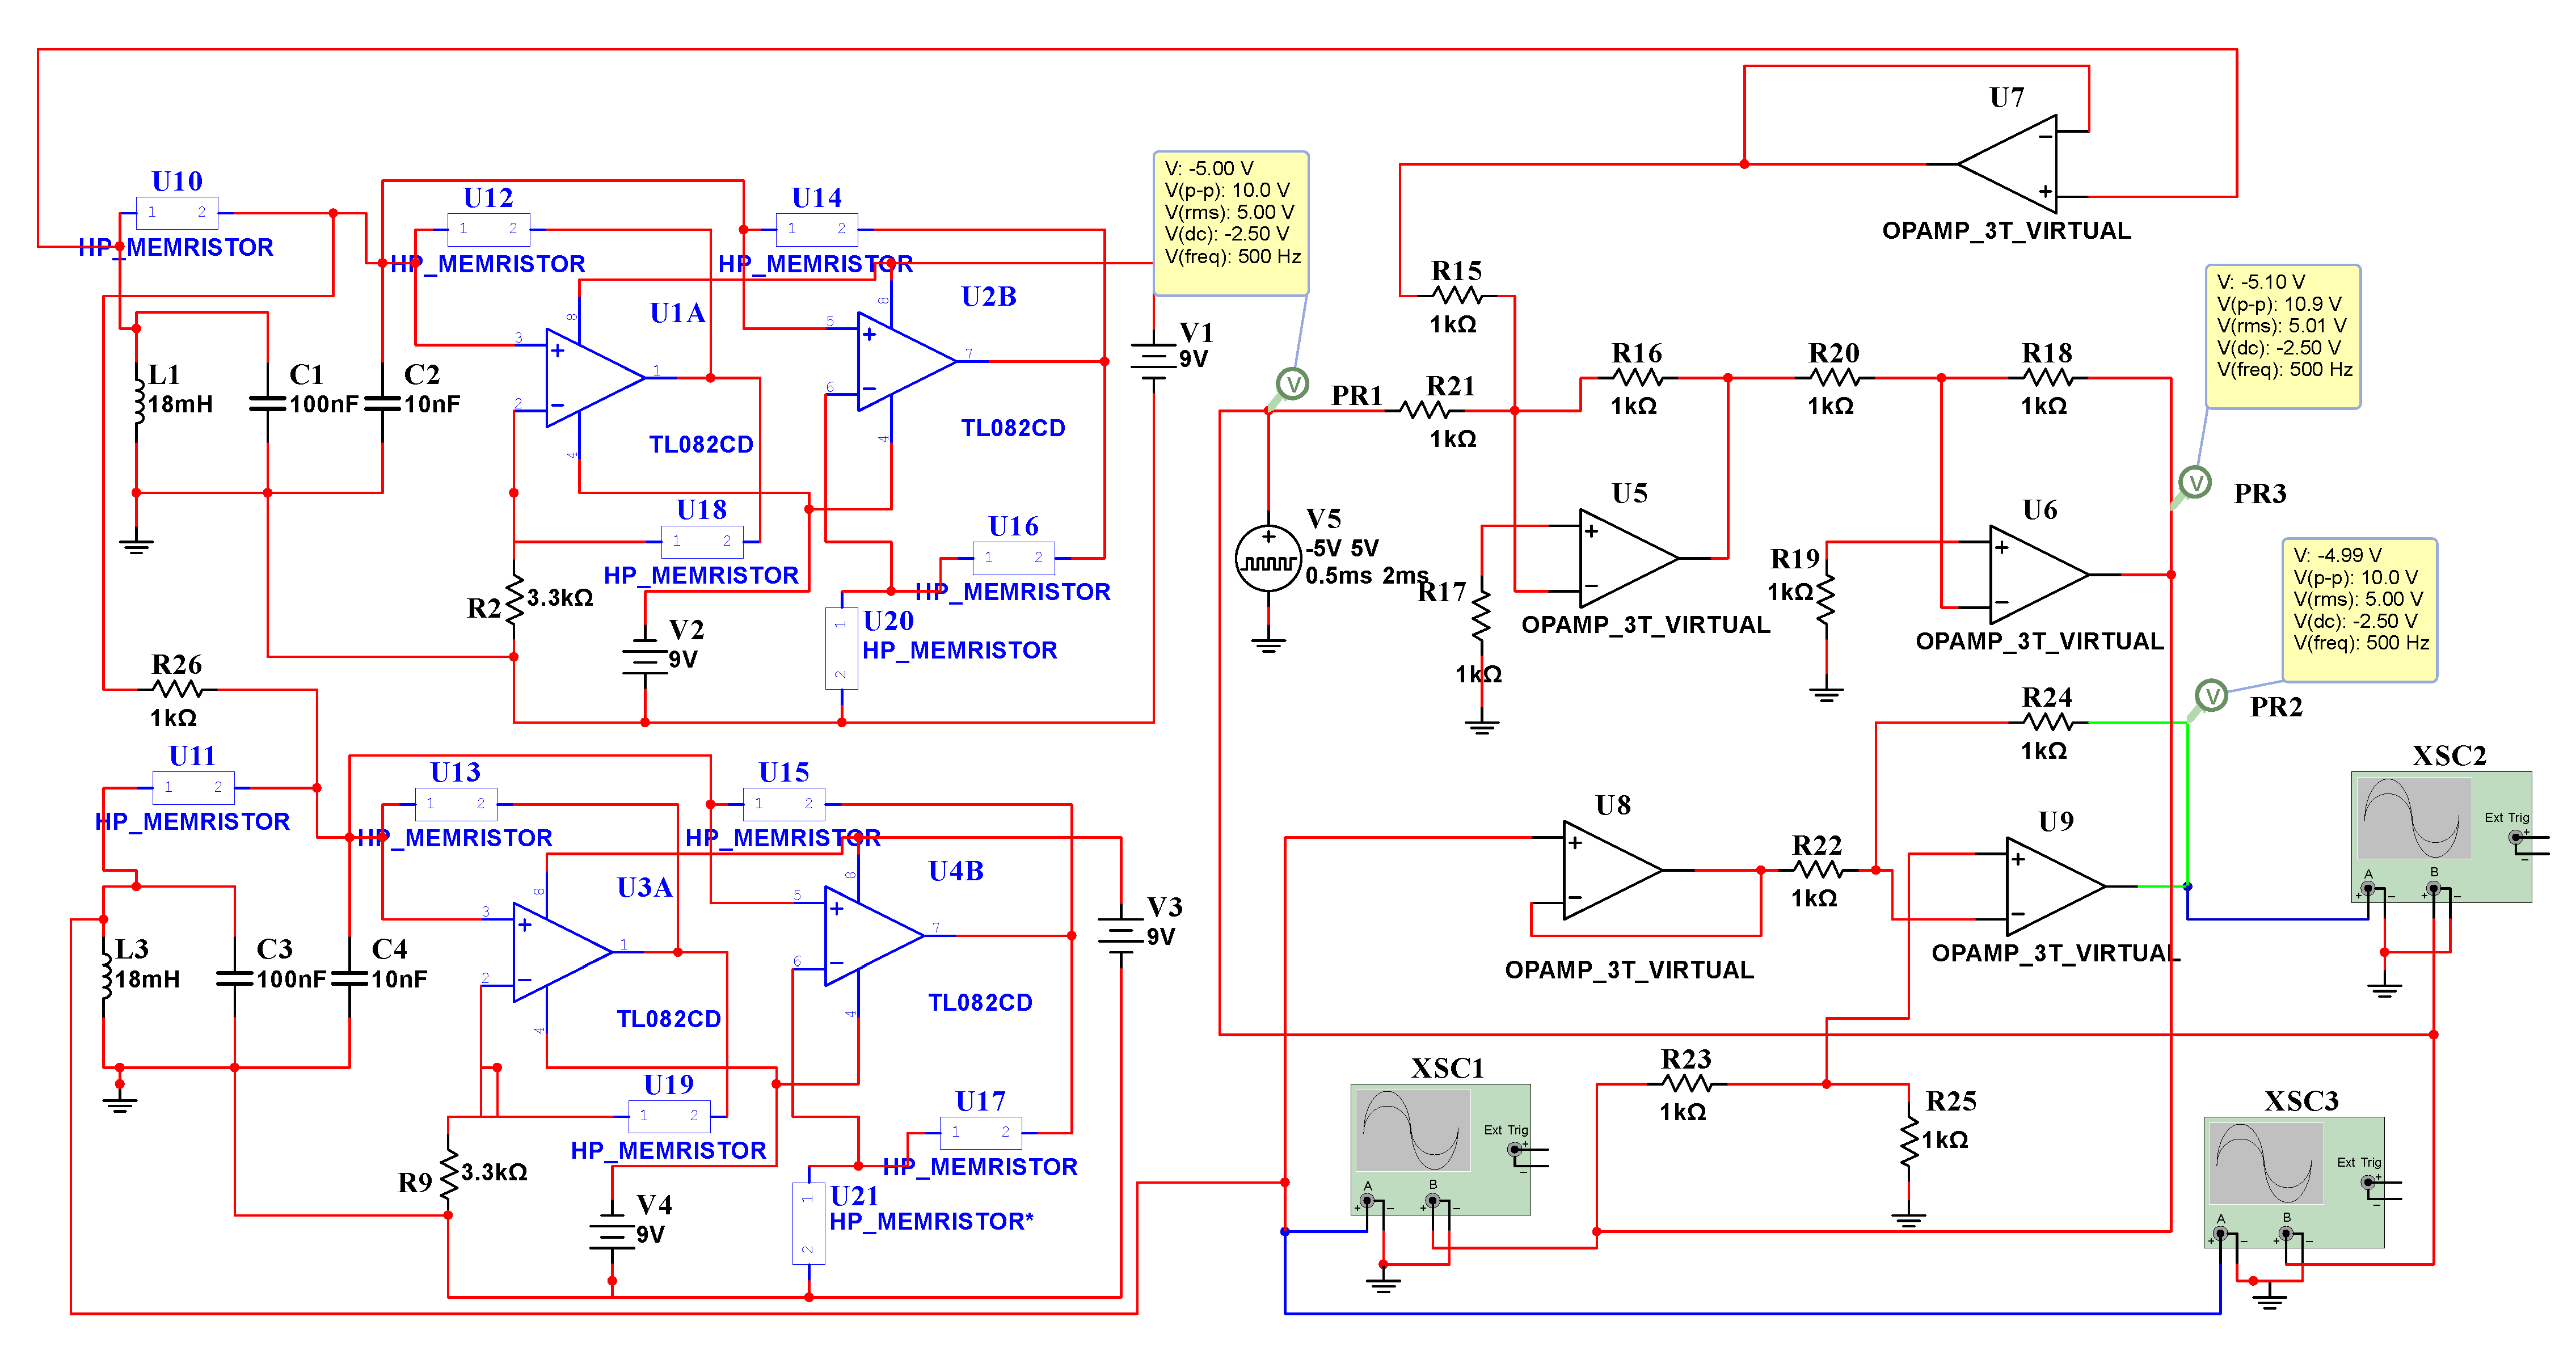
\includegraphics[width = 1\linewidth]{figs/Fig19multisim_Tx_Rx.PNG}
    \caption{Design of memristor-based Chua's chaotic circuit - non-identical transmitter and receiver}
    \label{fig:13}
\end{figure}

\begin{figure}[!t]
    \centering
    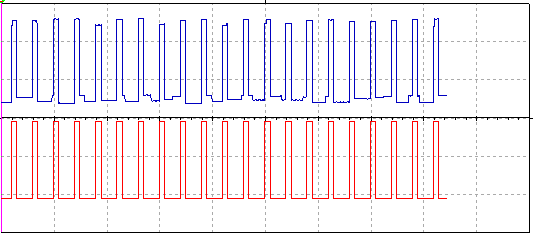
\includegraphics[width = 0.7\linewidth]{figs/Fig20x_OSC_02.PNG}
    \caption{Comparison of original message in red and decoded message in blue}
    \label{fig:14}
\end{figure}


The table below shows the values of the memristors used in the circuit of Fig. \ref{fig:13}, which remains same as Tx and Rx. Fig. \ref{fig:14} shows the original message is decoded successfully even when the circuit are non-identical. 

\begin{center}
\small
\begin{tabular}{|c c c |} 
 \hline
  &  & Memristor Parameters \\ [0.5ex] 
 \hline\hline
 Tx  & U10 & Ron=0.9K Roff=1.85K D=10N uv=10F p=1 \\ 
 \hline
 Rx & U11 & Ron=1K Roff=1.75K D=10N uv=10F p=1 \\ 
 \hline
\end{tabular}
\end{center}

\begin{center}
\small
\begin{tabular}{|c c c |} 
 \hline
 Tx & Rx & Memristor Parameters \\ [0.5ex] 
 \hline\hline
 U12 & U13 & Ron=11K Roff=22K D=10N uv=10F p=1 \\ 
 \hline
 U14 & U15 & Ron=110 Roff=220 D=10N uv=10F p=1 \\ 
 \hline
 U16 & U17 & Ron=110 Roff=220 D=10N uv=10F p=1 \\ 
 \hline
 U18 & U19 & Ron=11K Roff=22K D=10N uv=10F p=1 \\ 
 \hline
  U20 & U21 & Ron=1.1K Roff=2.2K D=10N uv=10F p=1 \\ 
 \hline
\end{tabular}
\end{center}

According to the above experiments, if the attacker discovers the correct key (i.e., the resistance of the memristors) within the range of $\Delta=0.1$, he/she may still decode the message; however, beyond this range, he/she has no luck. As a result, we take this value into account and employ the SMT attack \cite{9000113} on our proposed transceiver in Fig. \ref{fig:7}. We assume that the attacker has access to the prototyped receiver bought off the market and the transmitter design. The goal is to find the resistance of the memristors in such a way that the transmitter will be able to sync with the receiver. Each transmitter has six memristors; with $R_{max}$ set to 10K, each memristor can take $100,000$ different values resulting in $100,000^6$ cases which can be modeled with a key size of $100$ bits. We used 8GB of RAM and a 4-core processor at 2.20Ghz to run the attack. The attack, however, reports no key after 24 hours of running. This is due to the fact that the modeling of our analog logic locking circuit requires a large key space.


\section*{Discussion}

In this chapter, we presented a memristor-based chaotic transceiver designed to provide a robust defense against eavesdroppers and untrusted foundries. The efficacy of our approach lies in the creation of an extensive key space through the incorporation of memristors into the circuit, complemented by the implementation of logic locking. Validation of the proposed system was conducted through simulations in MATLAB Simulink, confirming the reliability and functionality of the memristor-based chaotic equations. This research holds particular relevance in enhancing the communication security of risk-sensitive implantable and wearable devices at the application level. By delivering a secure transceiver solution, our memristor-based chaotic system contributes significantly to fortifying the integrity of data transmission in these contexts.



\endgroup